\section{m-stitching and $\Pi$-m-stitching}

This section introduces key concepts that facilitate the construction of certified algorithms. 
It begins with the definitions of \textit{m-stitching} and \textit{$\Pi$-m-stitching}, 
followed by a presentation of the main theorem from 
Bumpus et al.~\cite{bumpus_et_al:LIPIcs.SWAT.2024.19}. 
These concepts and the theorem will be used for constructing certified algorithms 
in the following section. 
Unless stated otherwise, $\Pi$ is assumed to be a vertex-minimization problem.
We refer to the literature in \cite{bumpus_et_al:LIPIcs.SWAT.2024.19, venne2022designing}.

\subsection{FVS-4CL and 2-stitching}

The restriction we imposed on the Feedback Vertex Set problem enables us to look 
for optimal solutions in a local space. This is what m-stitching and $\Pi$-m-stitching
hint at. Here, the the variable $m$ is a positive integer that depends on the vertex optimization 
problem $\Pi$. In our case this is tied to the $\rho$ argument, i. e. the length of 
the cycles one is trying to break. 

To introduce $\Pi$-m-stitching, it is essential to first understand m-stitching 
and m-stitchable problems. In the stitching operation, two solutions $S_1$ and $S_2$ 
are given for a vertex optimization problem, along with an induced subgraph $J$ of $G$. 
Intuitively, the idea is to take the portion of $S_1$ that lies outside of $J$ 
and stitch onto it a suitable part of $S_2$ within the subgraph $J$.

The formal definition is as follows:

\refstepcounter{definition}
\begin{mydefinition}[m-stitching]{Def.}
    \label{m-stitch}

    Assume $m \geq 0$ is an integer, $J$ is an induced subgraph of $G$, and 
    $S_1, S_2 \subseteq V(G)$. Then we define the \textit{m-stitch} of $S_2$ onto $S_1$ along 
    $J$ as the set:

    \[S_3 := (S_1 \backslash J) \cup (S_2 \cap N^{m}_{G} \left[J\right]).\]

\end{mydefinition}

\begin{figure}[H]
    \centering
    \begin{minipage}{0.50\textwidth}
        \centering
        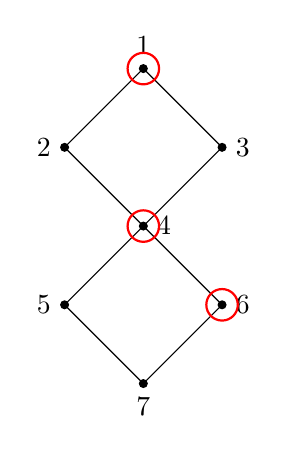
\begin{tikzpicture}
            % Define nodes
            \node[draw, circle, fill=black, scale=0.3, label=above:1] (1) at (0,2) {};
            \node[draw, circle, fill=black, scale=0.3, label=left:2] (2) at (-1,1) {};
            \node[draw, circle, fill=black, scale=0.3, label=right:3] (3) at (1,1) {};
            \node[draw, circle, fill=black, scale=0.3, label=right:4] (4) at (0,0) {};
            \node[draw, circle, fill=black, scale=0.3, label=left:5] (5) at (-1,-1) {};
            \node[draw, circle, fill=black, scale=0.3, label=right:6] (6) at (1,-1) {};
            \node[draw, circle, fill=black, scale=0.3, label=below:7] (7) at (0,-2) {};

            % Draw edges
            \draw (1) -- (2);
            \draw (1) -- (3);
            \draw (2) -- (4);
            \draw (3) -- (4);
            \draw (4) -- (5);
            \draw (4) -- (6);
            \draw (5) -- (7);
            \draw (6) -- (7);


            \draw[red, thick] (1) circle(0.2);
            \draw[red, thick] (4) circle(0.2);
            \draw[red, thick] (6) circle(0.2);

        \end{tikzpicture}
        \caption{Vertex set $S_1$}
    \end{minipage}
    \hfill
    \begin{minipage}{0.49\textwidth}
        \centering
        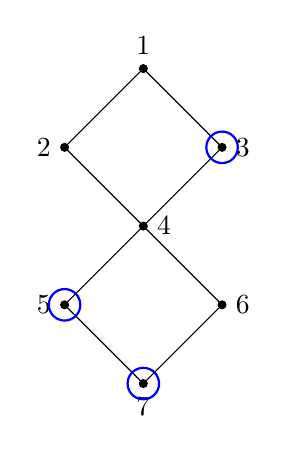
\begin{tikzpicture}
            % Define nodes
            \node[draw, circle, fill=black, scale=0.3, label=above:1] (1) at (0,2) {};
            \node[draw, circle, fill=black, scale=0.3, label=left:2] (2) at (-1,1) {};
            \node[draw, circle, fill=black, scale=0.3, label=right:3] (3) at (1,1) {};
            \node[draw, circle, fill=black, scale=0.3, label=right:4] (4) at (0,0) {};
            \node[draw, circle, fill=black, scale=0.3, label=left:5] (5) at (-1,-1) {};
            \node[draw, circle, fill=black, scale=0.3, label=right:6] (6) at (1,-1) {};
            \node[draw, circle, fill=black, scale=0.3, label=below:7] (7) at (0,-2) {};

            % Draw edges
            \draw (1) -- (2);
            \draw (1) -- (3);
            \draw (2) -- (4);
            \draw (3) -- (4);
            \draw (4) -- (5);
            \draw (4) -- (6);
            \draw (5) -- (7);
            \draw (6) -- (7);

            \draw[blue, thick] (3) circle(0.2);
            \draw[blue, thick] (5) circle(0.2);
            \draw[blue, thick] (7) circle(0.2);

        \end{tikzpicture}
        \caption{Vertex set $S_2$}
    \end{minipage}
\end{figure}

 In the following we show the subgraph $J$ we have chosen and the 2-neighbourhood 
of the subgraph.

 Also, in Fig.~\ref{fig:remove_s1} we show the first step of the m-stitch operation, namely 
removing the vertices of $J$ from the set $S_1$.

\begin{figure}[H]
    \centering
    \begin{minipage}{0.50\textwidth}
        \centering
        \begin{tikzpicture}
            % Define nodes
            \node[draw, circle, fill=black, scale=0.3, label=above:1] (1) at (0,2) {};
            \node[draw, circle, fill=black, scale=0.3, label=left:2] (2) at (-1,1) {};
            \node[draw, circle, fill=black, scale=0.3, label=right:3] (3) at (1,1) {};
            \node[draw, circle, fill=black, scale=0.3, label=right:4] (4) at (0,0) {};
            \node[draw, circle, fill=black, scale=0.3, label=left:5] (5) at (-1,-1) {};
            \node[draw, circle, fill=black, scale=0.3, label=right:6] (6) at (1,-1) {};
            \node[draw, circle, fill=black, scale=0.3, label=below:7] (7) at (0,-2) {};

            % Draw edges
            \draw (1) -- (2);
            \draw (1) -- (3);
            \draw (2) -- (4);
            \draw (3) -- (4);
            \draw (4) -- (5);
            \draw (4) -- (6);
            \draw (5) -- (7);
            \draw (6) -- (7);

            \begin{scope}[on background layer]
                \filldraw[orange!70,line width=20pt,rounded corners=5pt] (2.center) -- (3.center) -- (6.center) -- (7.center) -- (5.center) -- cycle;
            \end{scope}

            \begin{scope}[on background layer]   
                \filldraw[orange!35,line width=20pt,rounded corners=5pt] (6.center) --  (7.center) -- cycle;
            \end{scope}

        \end{tikzpicture}
        \caption{Subgraph $J$ of $G$ in light orange and $N^{2}_{G}\left[J\right]$ in darker orange}
    \end{minipage}
    \hfill
    \begin{minipage}{0.49\textwidth}
        \centering
        \begin{tikzpicture}
            % Define nodes
            \node[draw, circle, fill=black, scale=0.3, label=above:1] (1) at (0,2) {};
            \node[draw, circle, fill=black, scale=0.3, label=left:2] (2) at (-1,1) {};
            \node[draw, circle, fill=black, scale=0.3, label=right:3] (3) at (1,1) {};
            \node[draw, circle, fill=black, scale=0.3, label=right:4] (4) at (0,0) {};
            \node[draw, circle, fill=black, scale=0.3, label=left:5] (5) at (-1,-1) {};
            \node[draw, circle, fill=black, scale=0.3, label=right:6] (6) at (1,-1) {};
            \node[draw, circle, fill=black, scale=0.3, label=below:7] (7) at (0,-2) {};

            % Draw edges
            \draw (1) -- (2);
            \draw (1) -- (3);
            \draw (2) -- (4);
            \draw (3) -- (4);
            \draw (4) -- (5);
            \draw (4) -- (6);
            \draw (5) -- (7);
            \draw (6) -- (7);

            \begin{scope}[on background layer]   
                \filldraw[orange!70,line width=20pt,rounded corners=5pt] (2.center) -- (3.center) -- (6.center) -- (7.center) -- (5.center) -- cycle;
            \end{scope}

            \begin{scope}[on background layer]   
                \filldraw[orange!35,line width=20pt,rounded corners=5pt] (6.center) --  (7.center) -- cycle;
            \end{scope}

            \draw[red, thick] (1) circle(0.2);
            \draw[red, thick] (4) circle(0.2);

        \end{tikzpicture}
        \caption{Remove $J$ from $S_1$}
        \label{fig:remove_s1}
    \end{minipage}
\end{figure}

 What follows is the second step in obtaining set $S_3$ in Fig.~\ref{fig:second_step} and the 
stitched set in Fig.~\ref{fig:stitched_set}.

\begin{figure}[H]
    \centering
    \begin{minipage}{0.50\textwidth}
        \centering
        \begin{tikzpicture}
            % Define nodes
            \node[draw, circle, fill=black, scale=0.3, label=above:1] (1) at (0,2) {};
            \node[draw, circle, fill=black, scale=0.3, label=left:2] (2) at (-1,1) {};
            \node[draw, circle, fill=black, scale=0.3, label=right:3] (3) at (1,1) {};
            \node[draw, circle, fill=black, scale=0.3, label=right:4] (4) at (0,0) {};
            \node[draw, circle, fill=black, scale=0.3, label=left:5] (5) at (-1,-1) {};
            \node[draw, circle, fill=black, scale=0.3, label=right:6] (6) at (1,-1) {};
            \node[draw, circle, fill=black, scale=0.3, label=below:7] (7) at (0,-2) {};

            % Draw edges
            \draw (1) -- (2);
            \draw (1) -- (3);
            \draw (2) -- (4);
            \draw (3) -- (4);
            \draw (4) -- (5);
            \draw (4) -- (6);
            \draw (5) -- (7);
            \draw (6) -- (7);

            \begin{scope}[on background layer]   
                \filldraw[orange!70,line width=20pt,rounded corners=5pt] (2.center) -- (3.center) -- (6.center) -- (7.center) -- (5.center) -- cycle;
            \end{scope}

            \begin{scope}[on background layer]   
                \filldraw[orange!35,line width=20pt,rounded corners=5pt] (6.center) --  (7.center) -- cycle;
            \end{scope}

            \draw[red, thick] (1) circle(0.2);
            \draw[red, thick] (4) circle(0.2);

            \draw[blue, thick] (3) circle(0.2);
            \draw[blue, thick] (5) circle(0.2);
            \draw[blue, thick] (7) circle(0.2);


        \end{tikzpicture}
        \caption{Add $S_2 \cap N^{2}_{G} \left[J\right]$}
        \label{fig:second_step}
    \end{minipage}
    \hfill
    \begin{minipage}{0.49\textwidth}
        \centering
        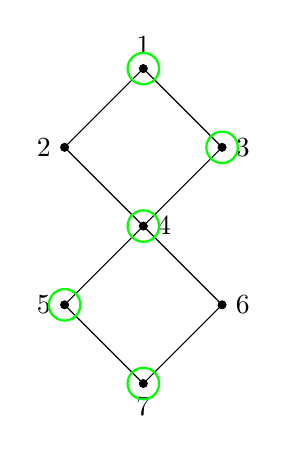
\begin{tikzpicture}
            % Define nodes
            \node[draw, circle, fill=black, scale=0.3, label=above:1] (1) at (0,2) {};
            \node[draw, circle, fill=black, scale=0.3, label=left:2] (2) at (-1,1) {};
            \node[draw, circle, fill=black, scale=0.3, label=right:3] (3) at (1,1) {};
            \node[draw, circle, fill=black, scale=0.3, label=right:4] (4) at (0,0) {};
            \node[draw, circle, fill=black, scale=0.3, label=left:5] (5) at (-1,-1) {};
            \node[draw, circle, fill=black, scale=0.3, label=right:6] (6) at (1,-1) {};
            \node[draw, circle, fill=black, scale=0.3, label=below:7] (7) at (0,-2) {};

            % Draw edges
            \draw (1) -- (2);
            \draw (1) -- (3);
            \draw (2) -- (4);
            \draw (3) -- (4);
            \draw (4) -- (5);
            \draw (4) -- (6);
            \draw (5) -- (7);
            \draw (6) -- (7);

            \draw[green, thick] (1) circle(0.2);
            \draw[green, thick] (3) circle(0.2);
            \draw[green, thick] (4) circle(0.2);
            \draw[green, thick] (5) circle(0.2);
            \draw[green, thick] (7) circle(0.2);

        \end{tikzpicture}
        \caption{Set $S_3$}
        \label{fig:stitched_set}
    \end{minipage}
\end{figure}

 A problem $\Pi$ is \textit{m-stitchable} if the set of feasible solutions are closed 
under the m-stitching operator. We hope that when we take the union in \ref{m-stitch} and arrive 
at the set $S_3$, this would too be a feasible solution.

\refstepcounter{definition}
\begin{mydefinition}[m-stitchable]{Def.}
    \label{m-stitchable}

    For an integer $m \geq 0$, induced subgraph $J$ and feasible solutions $S_1, S_2 \subseteq V(G)$ 
    of a vertex optimization problem $\Pi$ we have that the m-stitching of $S_2$ onto $S_1$ along 
    $J$, $S_3$ is a feasible solution to $\Pi$ on $G$.

    \[S_3 := (S_1 \backslash J) \cup (S_2 \cap N^{m}_{G} \left[J\right]).\]

\end{mydefinition}

 Now that we have a definition for problems $\Pi$ that are m-stitchable, we introduce 
$\Pi$-m-stitching as defined in \cite{bumpus_et_al:LIPIcs.SWAT.2024.19} and afterwards apply 
it to the current problem.

\refstepcounter{definition}
\begin{mydefinition}[$\Pi$-m-stitching]{Algorithm.}
    \label{alg:p-m-stitching}

    \textbf{Input:}
    an instance ($G, w : V(G) \to \mathbb{N}$) to an m-stitchable vertex optimization problem $\Pi$ 
    along with a solution $S_1$ and a vertex set $J \subseteq V(G)$.

    \textbf{Task:}
    find a feasible solution $S^{\prime}$ to $\Pi$ on $G$, such that for all other feasible solutions 
    $S^*$ it holds that $w(S^{\prime}) \leq w\left(S^{*} \oplus^{2}_{G,J} S_1\right)$.

\end{mydefinition}

 Before we proceed with the main theorem that we use to construct a certified algorithm 
we need one more definition.

\refstepcounter{definition}
\begin{mydefinition}[Guessable]{Def.}
    \label{guessable}

     A problem $\Pi$ is guessable if there is an algorithm that outputs a feasible solution 
    with no requirement for optimality in polynomial time.

\end{mydefinition}

 The following theorem is the main result in 
Bumpus et al.~\cite[Theorem 1.7]{bumpus_et_al:LIPIcs.SWAT.2024.19}.

\refstepcounter{definition}
\begin{mydefinition}[Main Theorem]{Theorem.}
    \label{theorem-main}

    Let $\mathbb{G}$ be a minor-closed graph class whose local tree-width is bounded above by a linear 
    function of the form $g : r \to \lambda \cdot r$ (fixed $\lambda \in \mathbb{R}$ and $r \in \mathbb{N}$).
    If $\Pi$ is a vertex-minimization problem and it holds that:

    \begin{enumerate}
        \item $\Pi$ is guessable.
        \item $\Pi$ is m-stitchable.
        \item There exists an algorithm $A_{\Pi}$ which solves $\Pi$-m-stitching in time $f(t) \cdot  |V(G)|^{\mathbb{O}(1)}$,
        where t = $\tw$($G\left[N^{m}_{G}(J)\right]$) and $f$ is a computable function;
    \end{enumerate}

    then, for each $\epsilon > 0$ there is a $(1 + \epsilon)$-certified algorithm for $\Pi$ that 
    runs in time $f(\lambda \cdot m / \epsilon) \cdot \left|V(G)\right| ^ {\mathbb{O}(1)}$ 
    on any input $(G, w : V(G) \to \mathbb{N})$ with $G \in \mathbb{G}$ and 
    polynomially-bounded weights.

\end{mydefinition}

 The proof of theorem \ref{theorem-main} is beyond the scope of this paper. In this section 
we only apply the three steps, mentioned to the FVS-BCL problem without generalizing to other 
vertex-minimization problems. 

 Firstly, we take a look at the guessable property.

\refstepcounter{definition}
\begin{mydefinition}[FVS-BCL is guessable]{Lemma}
    \label{lemma-guessable}

     For any planar graph $G$, the set $V(G)$ is a feasible solution to FVS-BCL.

\end{mydefinition}


\begin{proof}
    The graph $G - X$, where $X$ is the set of all vertices $V(G)$, is the empty graph, 
    therefore there are no 4-cycles left, after selecting that set.
\end{proof}

\refstepcounter{definition}
\begin{mydefinition}[FVS-BCL is 2-stitchable]{Lemma}
    \label{lemma-m-stitchable}

     Let $(G, w)$ be any instance to the FVS-4CL problem, $J \subseteq V(G)$, some subset
    of the vertices in the graph 
    and $S_1$ and $S_2$ any two feasible solutions to the problem in $G$. Then the set $S_3$:
    \[S_3 := (S_1 \backslash J) \cup (S_2 \cap N^{2}_{G} \left[J\right]).\]
    
    is a feasible solution to the problem.


\end{mydefinition}

\begin{proof}

Let the vertices $\{v_1,v_2,v_3,v_4\}$ form a 4-cycle.
We inspect the possible cases for the 4-cycle $v_1 v_2 v_3 v_4$. In order 
to prove \ref{lemma-m-stitchable} we have to prove that there exists a $v \in \{v_1, v_2, v_3, v_4\}$,
such that $v \in S_3$. 

\begin{enumerate}[label=\textbf{•}]
    \item $\exists v^{\prime} \in \{v_1,v_2,v_3,v_4\}$, such that $v^{\prime} \in J$. We argue in three steps.

    \begin{enumerate}
        \item Because $S_2$ is a feasible solution, then $\exists v'' \in \{v_1, v_2, v_3, v_4\}$,
        such that $v'' \in S_2$.
        \item Because there $\exists v' \in \{v_1,v_2,v_3,v_4\} \in J$, then it also holds
        that $\forall  v''' \in \{v_1,v_2,v_3,v_4\}, v''' \in N^{2}_{G}[J]$. From that and the previous 
        point it follows that $v'' \in S_2 \cap N^{2}_{G}[J]$.
        \item Finally, $S_2 \cap N^{2}_{G}[J] \subseteq S_3$, therefore $v'' \in S_3$.
    \end{enumerate}

    \item $\forall v' \in \{v_1,v_2,v_3,v_4\}$, it holds that $v' \notin J$.
    This case follows from the feasibility of $S_1$.

    \begin{enumerate}
        \item Because $S_1$ is a feasible solution, then $\exists v'' \in \{v_1,v_2,v_3,v_4\}$,
        such that $v'' \in S_1$.
        \item From $\forall v' \in \{v_1,v_2,v_3,v_4\} \notin J$ and the previous point, it follows 
        that $v'' \in S_1 \backslash J$.
        \item Because $S_1 \backslash J \subseteq S_3$, then $v'' \in S_3$.
    \end{enumerate}

\end{enumerate}

\end{proof}

 Now we describe an algorithm to find a feasible solution of minimum weight.

\begin{algorithm}[H]
    \caption{Stitch-FVS-4CL}
    \label{alg:stitch-fvs-4cl}
    \begin{algorithmic}[1]
    \REQUIRE Vertex-weighted planar graph $(G, w:V(G) \to \mathbb{N})$, a feasible solution $S_1$ on $G$
    and a vertex set $J \subseteq V(G)$
    .
    \ENSURE a feasible solution $S'$ on $G$, such that for all other feasible solutions $S^{*}$, 
    we have $w(S') \leq w(S^{*} \oplus^{2}_{G,J} S_1)$. 
    \STATE Let $H \leftarrow G[N^{2}_{G}[J] \backslash (S_1 \backslash J)]$. \label{state:construct-H}
    \STATE Let $S_2$ be the output of algorithm $A$ on input $(H, w)$. \label{state:opt-solution}
    \IF{ $w(S_2 \oplus^{2}_{G,J} S_1) < w(S_1)$ }
        \RETURN $S_2 \oplus^{2}_{G,J} S_1$
    \ELSE
        \RETURN $S_1$
    \ENDIF
    \end{algorithmic}
\end{algorithm}

The algorithm $A$ on line~\ref{alg:stitch-fvs-4cl} refers to calling 
Algorithm~\ref{courcelle:rho} that takes as input a graph that has bounded treewidth.


\refstepcounter{definition}
\begin{mydefinition}[FVS-4CL-2-stitching]{Lemma}
    \label{lemma-stictch-fvs-4cl}

    Let $A$ be an algorithm that solves FVS-4CL on any vertex-weighted instance $(G, w : V(G) \to \mathbb{N})$
    in time $f(t) \cdot |V(G)|^{O(1)}$ where $t$ is the treewidth of $G$. 
    Then Algorithm~\ref{alg:stitch-fvs-4cl} solves 
    FVS-4CL-2-stitching in time $f(\tw) \cdot n^{\mathcal{O}(1)}$ where 
    $\tw$ is the treewidth of $N^{2}_{G}[J]$. 
    In the end of the lemma we argue about the exact running time of the algorithm.
    
\end{mydefinition}

Note that it is not obvious that the set $S_2 \oplus^{2}_{G,J} S_1$ is a feasible solution in $G$ as $S_2$ is not 
necessarily a feasible solution in $G$. If the last was the case, then the feasibility of the 
$S_2 \oplus^{2}_{G,J} S_1$ would follow from Lemma~\ref{lemma-m-stitchable}. Therefore we first prove 
feasibility of $S_2 \oplus^{2}_{G,J} S_1$. Afterwards, we prove that it is of minimum weight.

\begin{proof}
    
We prove the feasibility of $S_2 \oplus^{2}_{G,J} S_1$ by case analysis on any four vertices
that form a 4-cycle. Remember that $S_2 \oplus^{2}_{G,J} S_1 = (S_1 \backslash J) \cup (S_2 \cap N^{2}_{G}[J])$.

\begin{enumerate}
    \item $\forall v' \in \{v_1,v_2,v_3,v_4\}: v' \in V(G) \backslash J$.

    Firstly, because of the feasibility of $S_1$, there $\exists v'' \in \{v_1,v_2,v_3,v_4\}: v'' \in S_1$.

    Secondly, $\forall v' \in \{v_1, v_2, v_3, v_4\}$, it holds that $v' \in V(G) \backslash J$.

    Finally from the first two conditions, using the property $A \backslash B = A \cap B^c$, 
    it holds that $v'' \in S_1 \backslash J$. From this
    and $S_1 \backslash J \subseteq S_2 \oplus^{2}_{G,J} S_1$, it follows that $S_2 \oplus^{2}_{G,J} S_1$ is feasible in $G$.

    In Fig.~\ref{fig:first-figure} we show (a part of) an example graph $G$ and the feasible solution 
    $S_1$ for it. In Fig.~\ref{fig:second-figure}, one can see that 4-cycles that do not have vertices 
    in $J$, are a part of $S_1 \backslash J \subseteq S_2 \oplus^{2}_{G,J} S_1$. 

    \begin{figure}[H]
        \centering
        \begin{minipage}{0.50\textwidth}
            \centering
            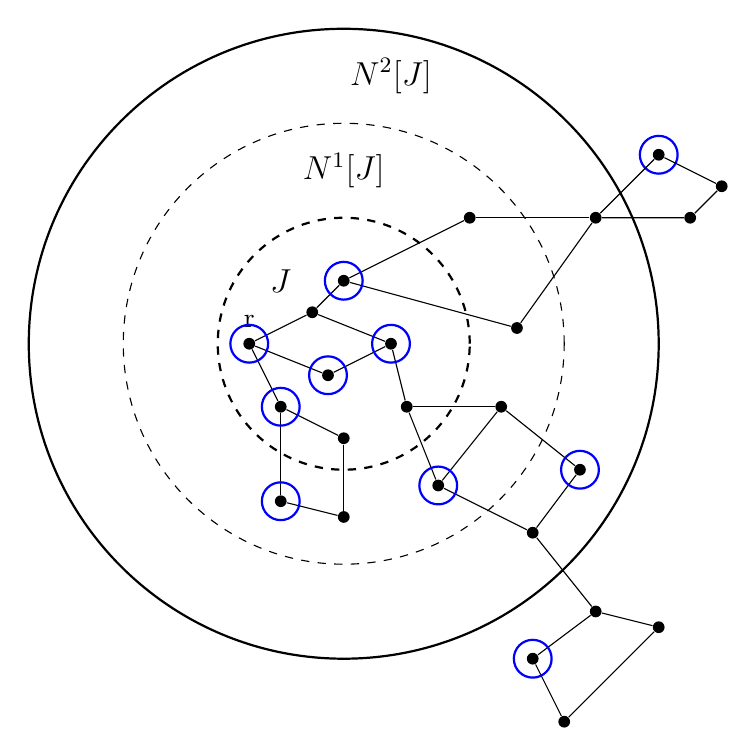
\begin{tikzpicture}[scale=0.8]
                %Draw J vertices
                \node[fill=black, circle, inner sep=1.5pt] (j01) at (0.75,0.5) {};
                \node[fill=black, circle, inner sep=1.5pt, label=above:r] (j02) at (-0.5,1) {};
                \node[fill=black, circle, inner sep=1.5pt] (j03) at (0.5,1.5) {};
                \node[fill=black, circle, inner sep=1.5pt] (j04) at (1.75,1) {};
        
                \node[fill=black, circle, inner sep=1.5pt] (j1) at (0,0) {};
                \node[fill=black, circle, inner sep=1.5pt] (j2) at (2,0) {};
                \node[fill=black, circle, inner sep=1.5pt] (j3) at (1,2) {};
                \node[fill=black, circle, inner sep=1.5pt] (j4) at (1,-0.5) {};
                
                % Draw N^1[J] vertices
        
                \node[fill=black, circle, inner sep=1.5pt] (n11) at (3.5,0) {};
                \node[fill=black, circle, inner sep=1.5pt] (n12) at (3.75,1.25) {};
                \node[fill=black, circle, inner sep=1.5pt] (n13) at (3,3) {};
                \node[fill=black, circle, inner sep=1.5pt] (n14) at (0,-1.5) {};
                \node[fill=black, circle, inner sep=1.5pt] (n15) at (1,-1.75) {};
                \node[fill=black, circle, inner sep=1.5pt] (n16) at (2.5,-1.25) {};
        
        
                % Draw N^2[J] vertices
                \node[fill=black, circle, inner sep=1.5pt] (n21) at (5, 3) {};
                \node[fill=black, circle, inner sep=1.5pt] (n22) at (4,-2) {};
                \node[fill=black, circle, inner sep=1.5pt] (n23) at (4.75,-1) {};
        
                % Draw vertices outside N^2[J]
                \node[fill=black, circle, inner sep=1.5pt] (n31) at (4, -4) {};
                \node[fill=black, circle, inner sep=1.5pt] (n32) at (5, -3.25) {};
                \node[fill=black, circle, inner sep=1.5pt] (n33) at (6, -3.5) {};
                \node[fill=black, circle, inner sep=1.5pt] (n34) at (4.5, -5) {};

                \node[fill=black, circle, inner sep=1.5pt] (new31) at (6, 4) {};
                \node[fill=black, circle, inner sep=1.5pt] (new32) at (6.5, 3) {};
                \node[fill=black, circle, inner sep=1.5pt] (new33) at (7, 3.5) {};
                
        
                % Draw edges inside J (induced subgraph)
                \draw (j01) -- (j02);
                \draw (j02) -- (j03);
                \draw (j03) -- (j04);
                \draw (j04) -- (j01);
        
                \draw (j4) -- (j1);

                \draw (j02) -- (j1);
                \draw (j04) -- (j2);
                \draw (j03) -- (j3);
                
                % Draw edges from J to N^1[J]
                \draw (j2) -- (n11);
                \draw (j2) -- (n16);
                \draw (j3) -- (n12);
                \draw (j1) -- (n14);
                \draw (j3) -- (n13);
                \draw (j4) -- (n15);
        
                % Draw edges inside N^1[J]
                \draw (n14) -- (n15);
                \draw (n16) -- (n11);
        
                % Draw edges between N^1[J] and N^2[J]
                \draw (n16) -- (n22);
                \draw (n11) -- (n23);
                \draw (n13) -- (n21);
                \draw (n12) -- (n21);
        
                % Draw edges between N^2[J] and N^2[J]
                \draw (n22) -- (n23);
        
                % Draw edges between N^2[J] and the other part of the graph
                \draw (n22) -- (n32);
        
                % Draw edges between the edges that are outside of N^2[J]
                \draw (n31) -- (n32);
                \draw (n32) -- (n33);
                \draw (n33) -- (n34);
                \draw (n34) -- (n31);
        
                % Draw the J circle
                \draw[dashed, thick] (1,1) circle [radius=2];
                \node at (0,2) {\large $J$};
        
                \draw[dashed] (1,1) circle [radius=3.5];
                \node at (1,3.75) {\large $N^1[J]$};
                
                % Draw the N^2[J] boundary as a larger circle
                \draw[thick] (1,1) circle [radius=5];
                \node at (1.75,5.25) {\large $N^2[J]$};
        
                % Draw vertices that are part of S_1
                \draw[blue, thick] (j01) circle(0.3);
                \draw[blue, thick] (j02) circle(0.3);
                \draw[blue, thick] (j04) circle(0.3);
        
                \draw[blue, thick] (j1) circle(0.3);
                \draw[blue, thick] (j3) circle(0.3);
                \draw[blue, thick] (n14) circle(0.3);
                \draw[blue, thick] (n16) circle(0.3);
                \draw[blue, thick] (n23) circle(0.3);
                \draw[blue, thick] (n31) circle(0.3);
                \draw[blue, thick] (new31) circle(0.3);

                \draw (n21) -- (new31);
                \draw (n21) -- (new32);
                \draw (new31) -- (new33);
                \draw (new32) -- (new33);
        
        
        
                %%%%%%%%%%%%%%%%%%%%%%%%%%%%%%%%%%%%%%%%%%%%%
                %%%%%%%%%%%%%%%%%%%%%%%%%%%%%%%%%%%%%%%%%%%%%
                %%%%%%%%%%%%%%%%%%%%%%%%%%%%%%%%%%%%%%%%%%%%%
                %%%%%%%%%%%%%%%%%%%%%%%%%%%%%%%%%%%%%%%%%%%%%
                %%%%%%%%%%%%%%%%%%%%%%%%%%%%%%%%%%%%%%%%%%%%%
                %%%%%%%%%%%%%%%%%%%%%%%%%%%%%%%%%%%%%%%%%%%%%
                %%%%%%%%%%%%%%%%%%%%%%%%%%%%%%%%%%%%%%%%%%%%%
                %%%%%%%%%%%%%%%%%%%%%%%%%%%%%%%%%%%%%%%%%%%%%
                %%%%%%%%%%%%%%%%%%%%%%%%%%%%%%%%%%%%%%%%%%%%%
                %%%%%%%%%%%%%%%%%%%%%%%%%%%%%%%%%%%%%%%%%%%%%
                %%%%%%%%%%%%%%%%%%%%%%%%%%%%%%%%%%%%%%%%%%%%%
                %%%%%%%%%%%%%%%%%%%%%%%%%%%%%%%%%%%%%%%%%%%%%
        
        
            \end{tikzpicture}
        \caption{Sets $J \subseteq N^{1}_{G}[J] \subseteq N^{2}_{G}[J] \subseteq G$;
        Feasible solution $S_1$ colored in blue.}
        \label{fig:first-figure}
        \end{minipage}
        \hfill
        \begin{minipage}{0.49\textwidth}
            \centering
            \begin{tikzpicture}[scale=0.8]
    
                %%%%%%%%%%%%%%%%%%%%%%%%%%%%%%%%%%%%%%%%%%%%%
                %%%%%%%%%%%%%%%%%%%%%%%%%%%%%%%%%%%%%%%%%%%%%
                %%%%%%%%%%%%%%%%%%%%%%%%%%%%%%%%%%%%%%%%%%%%%
                %%%%%%%%%%%%%%%%%%%%%%%%%%%%%%%%%%%%%%%%%%%%%
                %%%%%%%%%%%%%%%%%%%%%%%%%%%%%%%%%%%%%%%%%%%%%
                %%%%%%%%%%%%%%%%%%%%%%%%%%%%%%%%%%%%%%%%%%%%%
                %%%%%%%%%%%%%%%%%%%%%%%%%%%%%%%%%%%%%%%%%%%%%
                %%%%%%%%%%%%%%%%%%%%%%%%%%%%%%%%%%%%%%%%%%%%%
                %%%%%%%%%%%%%%%%%%%%%%%%%%%%%%%%%%%%%%%%%%%%%
                %%%%%%%%%%%%%%%%%%%%%%%%%%%%%%%%%%%%%%%%%%%%%
                %%%%%%%%%%%%%%%%%%%%%%%%%%%%%%%%%%%%%%%%%%%%%
                %%%%%%%%%%%%%%%%%%%%%%%%%%%%%%%%%%%%%%%%%%%%%
                
                %Draw J vertices
                \node[fill=black, circle, inner sep=1.5pt] (j01) at (0.75,0.5) {};
                \node[fill=black, circle, inner sep=1.5pt, label=above:r] (j02) at (-0.5,1) {};
                \node[fill=black, circle, inner sep=1.5pt] (j03) at (0.5,1.5) {};
                \node[fill=black, circle, inner sep=1.5pt] (j04) at (1.75,1) {};
    
                \node[fill=black, circle, inner sep=1.5pt] (j1) at (0,0) {};
                \node[fill=black, circle, inner sep=1.5pt] (j2) at (2,0) {};
                \node[fill=black, circle, inner sep=1.5pt] (j3) at (1,2) {};
                \node[fill=black, circle, inner sep=1.5pt] (j4) at (1,-0.5) {};
                
                % Draw N^1[J] vertices
    
                \node[fill=black, circle, inner sep=1.5pt] (n11) at (3.5,0) {};
                \node[fill=black, circle, inner sep=1.5pt] (n12) at (3.75,1.25) {};
                \node[fill=black, circle, inner sep=1.5pt] (n13) at (3,3) {};
                \node[fill=black, circle, inner sep=1.5pt] (n14) at (0,-1.5) {};
                \node[fill=black, circle, inner sep=1.5pt] (n15) at (1,-1.75) {};
                \node[fill=black, circle, inner sep=1.5pt] (n16) at (2.5,-1.25) {};
    
    
                % Draw N^2[J] vertices
                \node[fill=black, circle, inner sep=1.5pt] (n21) at (5, 3) {};
                \node[fill=black, circle, inner sep=1.5pt] (n22) at (4,-2) {};
                \node[fill=black, circle, inner sep=1.5pt] (n23) at (4.75,-1) {};
    
                % Draw vertices outside N^2[J]
                \node[fill=black, circle, inner sep=1.5pt] (n31) at (4, -4) {};
                \node[fill=black, circle, inner sep=1.5pt] (n32) at (5, -3.25) {};
                \node[fill=black, circle, inner sep=1.5pt] (n33) at (6, -3.5) {};
                \node[fill=black, circle, inner sep=1.5pt] (n34) at (4.5, -5) {};

                \node[fill=black, circle, inner sep=1.5pt] (new31) at (6, 4) {};
                \node[fill=black, circle, inner sep=1.5pt] (new32) at (6.5, 3) {};
                \node[fill=black, circle, inner sep=1.5pt] (new33) at (7, 3.5) {};
    
                % Draw edges inside J (induced subgraph)
                \draw (j01) -- (j02);
                \draw (j02) -- (j03);
                \draw (j03) -- (j04);
                \draw (j04) -- (j01);
    
                \draw (j4) -- (j1);

                \draw (j02) -- (j1);
                \draw (j04) -- (j2);
                \draw (j03) -- (j3);
                
                % Draw edges from J to N^1[J]
                \draw (j2) -- (n11);
                \draw (j2) -- (n16);
                \draw (j3) -- (n12);
                \draw (j1) -- (n14);
                \draw (j3) -- (n13);
                \draw (j4) -- (n15);
    
                % Draw edges inside N^1[J]
                \draw (n14) -- (n15);
                \draw (n16) -- (n11);
    
                % Draw edges between N^1[J] and N^2[J]
                \draw (n16) -- (n22);
                \draw (n11) -- (n23);
                \draw (n13) -- (n21);
                \draw (n12) -- (n21);
    
                % Draw edges between N^2[J] and N^2[J]
                \draw (n22) -- (n23);
    
                % Draw edges between N^2[J] and the other part of the graph
                \draw (n22) -- (n32);
    
                % Draw edges between the edges that are outside of N^2[J]
                \draw (n31) -- (n32);
                \draw (n32) -- (n33);
                \draw (n33) -- (n34);
                \draw (n34) -- (n31);

                \draw (n21) -- (new31);
                \draw (n21) -- (new32);
                \draw (new31) -- (new33);
                \draw (new32) -- (new33);
    
                % Draw the J circle
                \draw[dashed, thick] (1,1) circle [radius=2];
                \node at (0,2) {\large $J$};
    
                % Draw the N^2[J] boundary as a larger circle
                \draw[thick] (1,1) circle [radius=5];
                \node at (1.75,5.25) {\large $N^2[J]$};
    
                % Draw vertices that are part of S_1
                \draw[blue, thick] (j01) circle(0.3);
                \draw[blue, thick] (j02) circle(0.3);
                \draw[blue, thick] (j04) circle(0.3);
    
                \draw[blue, thick] (j1) circle(0.3);
                \draw[blue, thick] (j3) circle(0.3);
                \draw[blue, thick] (n14) circle(0.3);
                \draw[blue, thick] (n16) circle(0.3);
                \draw[blue, thick] (n23) circle(0.3);
                \draw[blue, thick] (n31) circle(0.3);
                \draw[blue, thick] (new31) circle(0.3);
    
                \begin{scope}[on background layer]   
                    \filldraw[orange!35,line width=15pt,rounded corners=5pt] (n31.center) -- (n32.center) -- (n33.center) -- (n34.center) -- cycle;
                \end{scope}
    
                \begin{scope}[on background layer]   
                    \filldraw[orange!35,line width=15pt,rounded corners=5pt] (n22.center) -- (n23.center) -- (n11.center) -- (n16.center) -- cycle;
                \end{scope}

                \begin{scope}[on background layer]   
                    \filldraw[orange!35,line width=15pt,rounded corners=5pt] (n21.center) -- (new31.center) -- (new33.center) -- (new32.center) -- cycle;
                \end{scope}
    
            \end{tikzpicture}
            \caption{$\forall v \in \{v_1,v_2,v_3,v_4\}: v \notin J$}
            \label{fig:second-figure}
        \end{minipage}
    \end{figure}


    \item $\exists v' \in \{v_1,v_2,v_3,v_4\}: v' \in J$. This also means that in this case 
    $\forall v' \in \{v_1,v_2,v_3,v_4\}: v' \in N^{2}_{G}[J]$.
    There are two cases to consider again. We know there $\exists v'' \in \{v_1,v_2,v_3,v_4\}$, 
    such that $v'' \in S_1$, we still have not considered whether or not it is a part of $J$.

    \begin{enumerate}
        \item $\exists v \in S_1: v \notin J$:
        
        In this case we can directly apply the previous point. From the properties of the set 
        difference operator we get: $v \in S_1 \backslash J \subseteq S_2 \oplus^{2}_{G,J} S_1$. 
        Consult Fig.~\ref{fig:third-figure} to see that there exists a vertex $v_{1,4}$ that is a part of 
        the 4-cycle, $v_{1,4} \notin J$, therefore $v_{1,4} \in S_1 \backslash J \subseteq S_2 \oplus^{2}_{G,J} S_1$.
        This means that in the new set $v_{1,4}$ will break that cycle.

        \item $\forall v \in S_1: v \in J$:

        In line~\ref{state:construct-H} of Algorithm~\ref{alg:stitch-fvs-4cl}, we have the following 
        construction of $H \leftarrow G[N^{2}_{G}[J] \backslash (S_1 \backslash J)]$. 

        \begin{align}
            V(H) &= N^{2}_{G}[J] \backslash (S_1 \backslash J) \\
                 &= N^{2}_{G}[J] \cap J \cup (N^{2}_G[J] \backslash S_1) \\
                 &= J \cup (N^{2}_G[J] \backslash S_1)
        \end{align}

        However, $\forall v \in \{v_1,v_2,v_3,v_4\}: v \in S_1 \land v \in J$. 
        Therefore $\{v_1,v_2,v_3,v_4\} \subseteq V(H)$. This means that in line~\ref{state:opt-solution} of 
        Algorithm~\ref{alg:stitch-fvs-4cl} we will add some $v^{*} \in \{v_1,v_2,v_3,v_4\}$ to $S_2$.

        Therefore $v \in S_2$, which has the same meaning as $v \in S_2 \cap N^{2}_{G}[J]$,
        and because $S_2 \cap N^{2}_{G}[J] \subseteq S_2 \oplus^{2}_{G,J} S_1$, we get 
        $v \in S_2 \oplus^{2}_{G,J} S_1$.

        Consult Fig.~\ref{fig:fourth-figure}. 

    \end{enumerate}

    \begin{figure}[H]
        \centering
        \begin{minipage}{0.50\textwidth}
            \centering
            \begin{tikzpicture}[scale=0.8]
                %Draw J vertices
                \node[fill=black, circle, inner sep=1.5pt] (j01) at (0.75,0.5) {};
                \node[fill=black, circle, inner sep=1.5pt, label=above:r] (j02) at (-0.5,1) {};
                \node[fill=black, circle, inner sep=1.5pt] (j03) at (0.5,1.5) {};
                \node[fill=black, circle, inner sep=1.5pt] (j04) at (1.75,1) {};
        
                \node[fill=black, circle, inner sep=1.5pt] (j1) at (0,0) {};
                \node[fill=black, circle, inner sep=1.5pt] (j2) at (2,0) {};
                \node[fill=black, circle, inner sep=1.5pt] (j3) at (1,2) {};
                \node[fill=black, circle, inner sep=1.5pt] (j4) at (1,-0.5) {};
                
                % Draw N^1[J] vertices
        
                \node[fill=black, circle, inner sep=1.5pt] (n11) at (3.5,0) {};
                \node[fill=black, circle, inner sep=1.5pt] (n12) at (3.75,1.25) {};
                \node[fill=black, circle, inner sep=1.5pt] (n13) at (3,3) {};
                \node[fill=black, circle, inner sep=1.5pt, label=below:$v_{1,4}$]  at (0,-1.5) {};
                \node[fill=black, circle, inner sep=1.5pt] (n15) at (1,-1.75) {};
                \node[fill=black, circle, inner sep=1.5pt] (n16) at (2.5,-1.25) {};
        
        
                % Draw N^2[J] vertices
                \node[fill=black, circle, inner sep=1.5pt] (n21) at (5, 3) {};
                \node[fill=black, circle, inner sep=1.5pt] (n22) at (4,-2) {};
                \node[fill=black, circle, inner sep=1.5pt] (n23) at (4.75,-1) {};
        
                % Draw vertices outside N^2[J]
                \node[fill=black, circle, inner sep=1.5pt] (n31) at (4, -4) {};
                \node[fill=black, circle, inner sep=1.5pt] (n32) at (5, -3.25) {};
                \node[fill=black, circle, inner sep=1.5pt] (n33) at (6, -3.5) {};
                \node[fill=black, circle, inner sep=1.5pt] (n34) at (4.5, -5) {};

                \node[fill=black, circle, inner sep=1.5pt] (new31) at (6, 4) {};
                \node[fill=black, circle, inner sep=1.5pt] (new32) at (6.5, 3) {};
                \node[fill=black, circle, inner sep=1.5pt] (new33) at (7, 3.5) {};

                % Draw edges inside J (induced subgraph)
                \draw (j01) -- (j02);
                \draw (j02) -- (j03);
                \draw (j03) -- (j04);
                \draw (j04) -- (j01);
        
                \draw (j4) -- (j1);

                \draw (j02) -- (j1);
                \draw (j04) -- (j2);
                \draw (j03) -- (j3);
                
                % Draw edges from J to N^1[J]
                \draw (j2) -- (n11);
                \draw (j2) -- (n16);
                \draw (j3) -- (n12);
                \draw (j1) -- (n14);
                \draw (j3) -- (n13);
                \draw (j4) -- (n15);
        
                % Draw edges inside N^1[J]
                \draw (n14) -- (n15);
                \draw (n16) -- (n11);
        
                % Draw edges between N^1[J] and N^2[J]
                \draw (n16) -- (n22);
                \draw (n11) -- (n23);
                \draw (n13) -- (n21);
                \draw (n12) -- (n21);
        
                % Draw edges between N^2[J] and N^2[J]
                \draw (n22) -- (n23);
        
                % Draw edges between N^2[J] and the other part of the graph
                \draw (n22) -- (n32);
        
                % Draw edges between the edges that are outside of N^2[J]
                \draw (n31) -- (n32);
                \draw (n32) -- (n33);
                \draw (n33) -- (n34);
                \draw (n34) -- (n31);

                \draw (n21) -- (new31);
                \draw (n21) -- (new32);
                \draw (new31) -- (new33);
                \draw (new32) -- (new33);
        
                % Draw the J circle
                \draw[dashed, thick] (1,1) circle [radius=2];
                \node at (0,2) {\large $J$};
        
                % Draw the N^2[J] boundary as a larger circle
                \draw[thick] (1,1) circle [radius=5];
                \node at (1.75,5.25) {\large $N^2[J]$};
        
                % Draw vertices that are part of S_1
                \draw[blue, thick] (j01) circle(0.3);
                \draw[blue, thick] (j02) circle(0.3);
                \draw[blue, thick] (j04) circle(0.3);
        
                \draw[blue, thick] (j1) circle(0.3);
                \draw[blue, thick] (j3) circle(0.3);
                \draw[blue, thick] (n14) circle(0.3);
                \draw[blue, thick] (n16) circle(0.3);
                \draw[blue, thick] (n23) circle(0.3);
                \draw[blue, thick] (n31) circle(0.3);
                \draw[blue, thick] (new31) circle(0.3);
    
                \begin{scope}[on background layer]   
                    \filldraw[orange!35,line width=15pt,rounded corners=5pt] (j1.center) -- (n14.center) -- (n15.center) -- (j4.center) -- cycle;
                \end{scope}
        
                %%%%%%%%%%%%%%%%%%%%%%%%%%%%%%%%%%%%%%%%%%%%%
                %%%%%%%%%%%%%%%%%%%%%%%%%%%%%%%%%%%%%%%%%%%%%
                %%%%%%%%%%%%%%%%%%%%%%%%%%%%%%%%%%%%%%%%%%%%%
                %%%%%%%%%%%%%%%%%%%%%%%%%%%%%%%%%%%%%%%%%%%%%
                %%%%%%%%%%%%%%%%%%%%%%%%%%%%%%%%%%%%%%%%%%%%%
                %%%%%%%%%%%%%%%%%%%%%%%%%%%%%%%%%%%%%%%%%%%%%
                %%%%%%%%%%%%%%%%%%%%%%%%%%%%%%%%%%%%%%%%%%%%%
                %%%%%%%%%%%%%%%%%%%%%%%%%%%%%%%%%%%%%%%%%%%%%
                %%%%%%%%%%%%%%%%%%%%%%%%%%%%%%%%%%%%%%%%%%%%%
                %%%%%%%%%%%%%%%%%%%%%%%%%%%%%%%%%%%%%%%%%%%%%
                %%%%%%%%%%%%%%%%%%%%%%%%%%%%%%%%%%%%%%%%%%%%%
                %%%%%%%%%%%%%%%%%%%%%%%%%%%%%%%%%%%%%%%%%%%%%
    
        
            \end{tikzpicture}
        \caption{$\exists v \in S_1: v \notin J$ (Remember we are in the case 
        where $\exists v \in J$)}
        \label{fig:third-figure}
        \end{minipage}
        \hfill
        \begin{minipage}{0.49\textwidth}
            \centering
            \begin{tikzpicture}[scale=0.8]
    
                %%%%%%%%%%%%%%%%%%%%%%%%%%%%%%%%%%%%%%%%%%%%%
                %%%%%%%%%%%%%%%%%%%%%%%%%%%%%%%%%%%%%%%%%%%%%
                %%%%%%%%%%%%%%%%%%%%%%%%%%%%%%%%%%%%%%%%%%%%%
                %%%%%%%%%%%%%%%%%%%%%%%%%%%%%%%%%%%%%%%%%%%%%
                %%%%%%%%%%%%%%%%%%%%%%%%%%%%%%%%%%%%%%%%%%%%%
                %%%%%%%%%%%%%%%%%%%%%%%%%%%%%%%%%%%%%%%%%%%%%
                %%%%%%%%%%%%%%%%%%%%%%%%%%%%%%%%%%%%%%%%%%%%%
                %%%%%%%%%%%%%%%%%%%%%%%%%%%%%%%%%%%%%%%%%%%%%
                %%%%%%%%%%%%%%%%%%%%%%%%%%%%%%%%%%%%%%%%%%%%%
                %%%%%%%%%%%%%%%%%%%%%%%%%%%%%%%%%%%%%%%%%%%%%
                %%%%%%%%%%%%%%%%%%%%%%%%%%%%%%%%%%%%%%%%%%%%%
                %%%%%%%%%%%%%%%%%%%%%%%%%%%%%%%%%%%%%%%%%%%%%
                
                %Draw J vertices
                \node[fill=black, circle, inner sep=1.5pt] (j01) at (0.75,0.5) {};
                \node[fill=black, circle, inner sep=1.5pt, label=above:r] (j02) at (-0.5,1) {};
                \node[fill=black, circle, inner sep=1.5pt] (j03) at (0.5,1.5) {};
                \node[fill=black, circle, inner sep=1.5pt] (j04) at (1.75,1) {};
    
                \node[fill=black, circle, inner sep=1.5pt] (j1) at (0,0) {};
                \node[fill=black, circle, inner sep=1.5pt] (j2) at (2,0) {};
                \node[fill=black, circle, inner sep=1.5pt] (j3) at (1,2) {};
                \node[fill=black, circle, inner sep=1.5pt] (j4) at (1,-0.5) {};
                
                % Draw N^1[J] vertices
    
                \node[fill=black, circle, inner sep=1.5pt] (n11) at (3.5,0) {};
                \node[fill=black, circle, inner sep=1.5pt] (n12) at (3.75,1.25) {};
                \node[fill=black, circle, inner sep=1.5pt] (n13) at (3,3) {};
                \node[fill=black, circle, inner sep=1.5pt] (n14) at (0,-1.5) {};
                \node[fill=black, circle, inner sep=1.5pt] (n15) at (1,-1.75) {};
                \node[fill=black, circle, inner sep=1.5pt] (n16) at (2.5,-1.25) {};
    
    
                % Draw N^2[J] vertices
                \node[fill=black, circle, inner sep=1.5pt] (n21) at (5, 3) {};
                \node[fill=black, circle, inner sep=1.5pt] (n22) at (4,-2) {};
                \node[fill=black, circle, inner sep=1.5pt] (n23) at (4.75,-1) {};
    
                % Draw vertices outside N^2[J]
                \node[fill=black, circle, inner sep=1.5pt] (n31) at (4, -4) {};
                \node[fill=black, circle, inner sep=1.5pt] (n32) at (5, -3.25) {};
                \node[fill=black, circle, inner sep=1.5pt] (n33) at (6, -3.5) {};
                \node[fill=black, circle, inner sep=1.5pt] (n34) at (4.5, -5) {};

                \node[fill=black, circle, inner sep=1.5pt] (new31) at (6, 4) {};
                \node[fill=black, circle, inner sep=1.5pt] (new32) at (6.5, 3) {};
                \node[fill=black, circle, inner sep=1.5pt] (new33) at (7, 3.5) {};
    
                % Draw edges inside J (induced subgraph)
                \draw (j01) -- (j02);
                \draw (j02) -- (j03);
                \draw (j03) -- (j04);
                \draw (j04) -- (j01);
    
                \draw (j4) -- (j1);

                \draw (j02) -- (j1);
                \draw (j04) -- (j2);
                \draw (j03) -- (j3);
                
                % Draw edges from J to N^1[J]
                \draw (j2) -- (n11);
                \draw (j2) -- (n16);
                \draw (j3) -- (n12);
                \draw (j1) -- (n14);
                \draw (j3) -- (n13);
                \draw (j4) -- (n15);
    
                % Draw edges inside N^1[J]
                \draw (n14) -- (n15);
                \draw (n16) -- (n11);
    
                % Draw edges between N^1[J] and N^2[J]
                \draw (n16) -- (n22);
                \draw (n11) -- (n23);
                \draw (n13) -- (n21);
                \draw (n12) -- (n21);
    
                % Draw edges between N^2[J] and N^2[J]
                \draw (n22) -- (n23);
    
                % Draw edges between N^2[J] and the other part of the graph
                \draw (n22) -- (n32);
    
                % Draw edges between the edges that are outside of N^2[J]
                \draw (n31) -- (n32);
                \draw (n32) -- (n33);
                \draw (n33) -- (n34);
                \draw (n34) -- (n31);

                \draw (n21) -- (new31);
                \draw (n21) -- (new32);
                \draw (new31) -- (new33);
                \draw (new32) -- (new33);
    
                % Draw the J circle
                \draw[dashed, thick] (1,1) circle [radius=2];
                \node at (0,2) {\large $J$};
    
                % Draw the N^2[J] boundary as a larger circle
                \draw[thick] (1,1) circle [radius=5];
                \node at (1.75,5.25) {\large $N^2[J]$};
    
                % Draw vertices that are part of S_1
                \draw[blue, thick] (j01) circle(0.3);
                \draw[blue, thick] (j02) circle(0.3);
                \draw[blue, thick] (j04) circle(0.3);
    
                \draw[blue, thick] (j1) circle(0.3);
                \draw[blue, thick] (j3) circle(0.3);
                \draw[blue, thick] (n14) circle(0.3);
                \draw[blue, thick] (n16) circle(0.3);
                \draw[blue, thick] (n23) circle(0.3);
                \draw[blue, thick] (n31) circle(0.3);
                \draw[blue, thick] (new31) circle(0.3);
    
                \begin{scope}[on background layer]   
                    \filldraw[orange!35,line width=15pt,rounded corners=5pt] (j01.center) -- (j02.center) -- (j03.center) -- (j04.center) -- cycle;
                \end{scope}
    
                \begin{scope}[on background layer]   
                    \filldraw[orange!35,line width=15pt,rounded corners=5pt] (j3.center) -- (n12.center) -- (n21.center) -- (n13.center) -- cycle;
                \end{scope}
    
            \end{tikzpicture}
            \caption{$\forall v \in S_1: v \in J$}
            \label{fig:fourth-figure}
        \end{minipage}
    \end{figure}

\end{enumerate}

 The proof of optimality of the set $S_2 \oplus^{2}_{G,J} S_1$ is similar to the one in 
Bumpus et al.\cite[Lemma 3.2]{bumpus_et_al:LIPIcs.SWAT.2024.19}. It is important to note 
that we can use the same proof, because of a property of the FVS-4CL problem, namely that 
a 4-cycle breaking set is closed under taking induced subgraphs.

 Remember, we are still trying to prove what we mentioned in Algorithm~\ref{alg:p-m-stitching},
namely that some feasible solution $S'$ (which in our case is the $S_2 \oplus^{2}_{G,J} S_1$), is of minimum weight,
that is, for all other feasible solutions $S^{*}$, it holds that $w(S') \leq w(S^{*} \oplus^{2}_{G,J} S_1)$.

Assume by way of contradiction that there is a feasible solution $S_3$ for $G$,
such that $w(S_3 \oplus^{2}_{G,J} S_1) < w(S_2 \oplus^{2}_{G,J} S_1)$. Then it would follow that:

\[
\begin{aligned}
w|_{V(F)}(S_2) &= w(S_2) && \text{since } S_2 \subseteq V(F) \text{} \\
&= w(S_2 \cap N^{2}_{G}[J]) && \text{since } V(F) \subseteq N^{2}_{G}[J] \\
&= w(S_1 \setminus J) + w(S_2 \cap N^{2}_{G}[J]) - w(S_1 \setminus J)  \\
&= w((S_1 \setminus J) \cup (S_2 \cap N^{2}_{G}[J])) - w(S_1 \setminus J) && \text{since } V(F) \cap (S_1 \setminus J) = \emptyset \\
&= w(S_2 \oplus^{2}_{G,J} S_1) - w(S_1 \setminus J) && \text{by definition of stitch} \\
&> w(S_3 \oplus^{2}_{G,J} S_1) - w(S_1 \setminus J) && \text{by assumption on } S_3 \\
&= w((S_1 \setminus J) \cup (S_3 \cap N^{2}_{G}[J])) - w(S_1 \setminus J) && \text{by definition of stitch} \\
&= w((S_3 \cap N^{2}_{G}[J]) \setminus (S_1 \setminus J)) && \text{since } w(A \cup B) - w(A) = w(B \setminus A)  \\
&= w(S_3 \cap (N^{2}_{G}[J] \setminus (S_1 \setminus J))) && \text{since } (A \cap B) \setminus C = A \cap (B \setminus C)  \\
&= w(S_3 \cap V(F)) && \text{by definition of } F \\
&= w|_{V(F)}(S_3 \cap V(F))
\end{aligned}
\]
\end{proof}

\textbf{Running time:}

The running time of the algorithm is dominated by the call of algorithm $A$. For 
$\tw$, the treewidth of $N^{2}_{G}[J]$, 
the running time is 
$2^{\mathcal{O}(\tw^2)} \cdot n^{\mathcal{O}(1)}$. Here we use the dynamic programming algorithm (\ref{alg:dp}).

\subsection{FVS-BCL and ($\rho / 2$)-stitching}

In this subsection, we extend the results for FVS-4CL to the more general problem. 
In earlier sections, we showed that FVS-BCL admits an EPTAS by observing that 
$\lfloor \frac{\rho}{2} \rfloor$ layers of overlap between two subgraphs are sufficient for a 
$\rho$-cycle to be entirely contained within one of the subgraphs, possibly including the 
overlapping region (see Fig.~\ref{fig:bfs_tree}, \ref{fig:first-figure}). 
When applying the $m$-stitching technique, the reader should understand that the two relevant 
subgraphs are $G[V(G) \setminus J]$ and $G[J]$. If we construct an algorithm similar to 
Algorithm~\ref{alg:stitch-fvs-4cl} but set the parameter $m$ to 
$\lfloor \frac{\rho}{2} \rfloor$ instead of 2, the resulting algorithm solves 
FVS-BCL-stitching in time 
$f(\tw) \cdot n^{\mathcal{O}(1)}$ 
where $\tw$ is the treewidth of $N^{\lfloor\frac{\rho}{2}\rfloor}_{G}[J]$. 
It is important to note that a $\rho$-cycle breaking set is closed under taking 
induced subgraphs. This is another reason we can construct such an algorithm and do not 
have to take a different approach as we will do with the $r$-Dominating Set.

From the arguments in the previous paragraph we can infer that:

\begin{enumerate}
    \item FVS-BCL is $\lfloor\frac{\rho}{2}\rfloor$-stitchable.
    \item There exists an algorithm $A_{\text{FVS-BCL}}$ which solves 
    FVS-BCL-$\lfloor\frac{\rho}{2}\rfloor$-stitching in time 
    $f(\tw) \cdot n^{\mathcal{O}(1)}$ 
    where $\tw$ is the treewidth of any $N^{\lfloor\frac{\rho}{2}\rfloor}_{G}[J]$ and 
    $f$ is some computable function.
\end{enumerate}

The problem is also trivially guessable. Like in the FVS-4CL, taking the set $V(G)$, would 
break all $\rho$-cycles in a graph.

\textbf{Running time:}

For some computable function $f$, constant $\rho$ and $\tw$, treewidth of 
$N^{\lfloor\frac{\rho}{2}\rfloor}_{G}[J]$,
the algorithm we described solves 
FVS-BCL-$\rho$-stitching in time $f(\tw) \cdot n^{\mathcal{O}(1)}$.

\subsection{r-Dominating Set and $(r+1)$-stitching}

In this subsection we will use the definitions and terminology we have established in the 
previous section and look at another problem, namely the r-Dominating Set problem. We will 
argue that in the case of that problem the parameter $m$ has to be set to $r+1$ in order 
to maintain feasibility when constructing new sets. Afterwards we will prove that 
when constructing new sets, one can find a feasible solution which is also optimal. 
We follow the steps we established in the previous section.

Firstly, prove that the problem is guessable and m-stitchable. Secondly, devise an algorithm 
$A_{\text{r-DS}}$ that solves the problem in FPT. Finally, using Theorem~\ref{theorem-main}, 
prove that the problem is certified.

\refstepcounter{definition}
\begin{mydefinition}[\boldsymbol{$r$}-DS is guessable]{Lemma}
    \label{lemma-ds-guessable}

    For any planar graph $G$, the set $V(G)$ is a feasible solution to r-DS.

\end{mydefinition}

\begin{proof}
    Let $X$ be the set of all vertices in $G$, $X \leftarrow V(G)$. Therefore, it is 
    trivially true that $N^r_G[X] = V(G)$. 
\end{proof}

\refstepcounter{definition}
\begin{mydefinition}[r-DS is $(r+1)$-stitchable]{Lemma}
    \label{lemma-r-DS-stitchable}

    Let $(G, w)$ be any instance to the $r$-DS problem, $J \subseteq V(G)$, some subset
    of the vertices in the graph 
    and $S_1$ and $S_2$ any two feasible solutions to the problem in $G$. Then the set $S_3$:
    \[S_3 := (S_1 \backslash J) \cup (S_2 \cap N^{r+1}_{G} \left[J\right]).\]
    is a feasible solution to the problem.

\end{mydefinition}

\begin{proof}
    For a vertex $v \in V(G)$, we have the following cases:

    \begin{enumerate}
        \item $v \in V(G) \backslash N^{r+1}_{G}[J]$. Because $S_1$ is a feasible solution,
        it is clear that $v$ will be dominated by some vertex $u$ in $S_1 \backslash J$. Since 
        $S_1 \backslash J \subseteq S_3$, then $u \in S_3$.
        \item $v \in N^{r+1}_{G}[J]$. Because $S_2$ is a feasible solution, it is clear 
        that $S_2 \cap N^{r+1}_{G}[J]$ contains a vertex $u$ which dominates $v$. Since 
        $S_2 \cap N^{r+1}_{G}[J] \subseteq S_3$, then $u \in S_3$.
    \end{enumerate}

    In both cases we have argued that there $\exists u \in S_3$, such that for any vertex 
    $v \in V(G)$, $u$ dominates $v$.

\end{proof}

Now we describe an algorithm to find a feasible solution of minimum weight.

\begin{algorithm}[H]
    \caption{Stitch-r-DS}
    \label{alg:stitch-r-DS}
    \begin{algorithmic}[1]
    \REQUIRE Vertex-weighted planar graph $(G, w:V(G) \to \mathbb{N})$,
    a feasible solution of r-DS $S_1$ on $G$
    and a vertex set $J \subseteq V(G)$.
    \ENSURE a feasible solution $S'$ on $G$, such that for all other feasible solutions $S^{*}$, 
    we have $w(S') \leq w(S^{*} \oplus^{r+1}_{G,J} S_1)$. 
    \STATE Let $H \leftarrow G[N^{r+1}_{G}[J]] \cup \{q\}$, where for vertex $q$
    it holds that $N_H(q) := N_{G}(N^{r}_{G}[J])$ (Vertex $q$ is adjacent to the vertices 
    at distance exactly $r+1$ from $J$). \label{state:construct-H-rds}
    \STATE \[
    w_H(x) = 
    \begin{cases}
    0 & \text{if } x \in (S_1 \setminus J) \cup \{q\} \\
    w(x) & \text{otherwise}
    \end{cases}
    \]
    \STATE Let $S_2'$ be the output of algorithm $A$ on input $(H, w)$. 
    \STATE Let $S_2 = S_2' \backslash \{q\}$. \label{state:opt-solution-rds}
    \IF{ $w(S_2 \oplus^{r+1}_{G,J} S_1) < w(S_1)$ }
        \RETURN $S_2 \oplus^{r+1}_{G,J} S_1$
    \ELSE
        \RETURN $S_1$
    \ENDIF
    \end{algorithmic}
\end{algorithm}

\refstepcounter{definition}
\begin{mydefinition}[$r$-DS-$(r+1)$-stitching]{Lemma}
    \label{lemma-rds-stitching}

    Let $A$ be an algorithm that solves $r$-stitching on any vertex-weighted instance 
    $(G, w : V(G) \to \mathbb{N})$ in time $f(t) \cdot |V(G)|^{\mathcal{O}(1)}$ where 
    $t$ is the treewidth of $G$. Then 
    Algorithm~\ref{alg:stitch-r-DS} solves $r$-DS in time 
    $f(\tw) \cdot V(G)^{\mathcal{O}(1)}$ where $\tw$ is the treewidth of $(N^{r+1}_{G}[J])$.

\end{mydefinition}

The proof of Lemma~\ref{lemma-rds-stitching} is outside of the scope of this paper 
as it is similar to the proof of Lemma~\ref{lemma-stictch-fvs-4cl}. The reader can find 
a similar proof in Bumpus et al. \cite[Lemma 3.3]{bumpus_et_al:LIPIcs.SWAT.2024.19}.

\textbf{Running time:}

For some constant $r$ and $\tw$, the treewidth of $N^{r+1}_{G}[J]$, the running time of 
the algorithm is: $(2r+1)^{\tw + 1} \cdot \tw^{2} \cdot n^{\mathcal{O}(1)}$.